\documentclass{jarticle}

\setlength{\textwidth}{185mm}
\setlength{\textheight}{225mm}
\setlength{\topmargin}{0cm}
\setlength{\oddsidemargin}{-1cm}
\setlength{\evensidemargin}{-1cm}

\usepackage[dvipdfmx]{graphicx} %PDF用
\usepackage{eclbkbox} %breakbox用


\title{プログラム入門 レポート}
\author{琉球大学 工学部 情報工学科\\145770F 秋田 海人}
\date{}

\begin{document}
\maketitle
\parindent = 0pt


\section{第 I 章\\}
\subsection{問1-1\\}
\subsubsection{プログラム\\}
\begin{breakbox}
\begin{verbatim}
#include <stdio.h>

int main(void) {
	printf("Hello \n World!");
}
\end{verbatim}
\end{breakbox}
\subsubsection{実行結果\\}
\begin{breakbox}
\begin{verbatim}
Hello 
 World!
\end{verbatim}
\end{breakbox}
\subsubsection{考察\\}
\textbackslash{n}は改行を意味する特殊文字である。\\
printf("Hello \textbackslash{n} World!");を出力する時,Helloのあとに\textbackslash{n}があるので一度改行を行いそのあとにWorldを出力するプログラムになっている。\\
\newpage
\subsection{問1-2\\}
\begin{breakbox}
\begin{verbatim}
\a    警報音
\b    バックスペース
\n    復帰改行
\r    復帰
\f    改ページ
\t    水平タブ
\v    垂直タブ
\\   文字としての\
\?    文字としての?
\'    シングルクォーテーション(')
\"    ダブルクォーテーション(")
\0    Null(ヌル)
\ooo	    8進数の文字コードを持つ文字
\xhh	    16進数の文字コードを持つ文字
\end{verbatim}
\end{breakbox}
\subsubsection{考察\\}
\textbackslash{n},\textbackslash{t}は利用したことある。\\
\textbackslash{n}はよく使われるものである。\\
\textbackslash{t}は見やすさを配慮したい時に利用した経験がある。\\

\subsection{問1-3\\}
\subsubsection{プログラム\\}
\begin{breakbox}
\begin{verbatim}
#include <stdio.h>

int main(void) {
	int x, y, z;
	x = 5;
	y = 2;
	z = x - y;
	
	printf("Answer %d\n", z);
	printf("%d - %d = %d\n", x, y ,z);
}
\end{verbatim}
\end{breakbox}
\subsubsection{実行結果\\}
\begin{breakbox}
\begin{verbatim}
Answer 3
5 - 2 = 3
\end{verbatim}
\end{breakbox}
\subsubsection{考察\\}
上記の実行結果は整数値を入れ実行した。\\
するとただの5 - 2 = 3という結果が返ってくる。\\
これを小数にすると,変数の宣言でint型(整数型)を使っているので実数を用いるとエラーとなりコンパイルすらできなくなる。\\
非常に大きい値にすると,int型は-2,147,483,648 〜 2,147,483,647の範囲しか扱うことができないので,これ以上の値になるとエラーで実行することができなくなる。\\


\subsection{問1-4\\}
\subsubsection{プログラム\\}
\begin{breakbox}
\begin{verbatim}
#include <stdio.h>

int main(void) {
	int ax, ay, az;
	int bx, by, bz;
	int n, g_1, g_2, g_3;
  printf("Input ax, ay, az \n");
	scanf("%d %d %d", &ax ,&ay, &az);
  printf("Input bx, by, bz \n");
	scanf("%d %d %d", &bx ,&by, &bz);
  
	n = (ax * bx) + (ay * by) + (az * bz); 
	g_1 = (ay * bz) - (az * by); 
	g_2 = (az * bx) - (ax * bz); 
	g_3 = (ax * by) - (ay * bx);

	printf("内積: %d \n", n);
	printf("外積: (%d, %d, %d)\n", g_1, g_2, g_3); 
}
\end{verbatim}
\end{breakbox}
\subsubsection{実行結果\\}
\begin{breakbox}
\begin{verbatim}
Input ax, ay, az 
1 0 1
Input bx, by, bz 
1 1 0
内積: 1 
外積: (-1, 1, 1)
\end{verbatim}
\end{breakbox}
\subsubsection{考察\\}
整数をキボードから入力するようにした。\\
数式をそのままプログラムとして書き,出力は内積と外積がわかりやすいように工夫した。\\


\subsection{問1-5\\}
\subsubsection{プログラム\\}
\begin{breakbox}
\begin{verbatim}
#include <stdio.h>

int main(void) {
	double ax, ay, az;
	double bx, by, bz;
	double n, g_1, g_2, g_3;
  printf("Input ax, ay, az \n");
	scanf("%lf %lf %lf", &ax ,&ay, &az);
  printf("Input bx, by, bz \n");
	scanf("%lf %lf %lf", &bx ,&by, &bz);
  
	n = (ax * bx) + (ay * by) + (az * bz); 
	g_1 = (ay * bz) - (az * by); 
	g_2 = (az * bx) - (ax * bz); 
	g_3 = (ax * by) - (ay * bx);

	printf("内積: %lf \n", n);
	printf("外積: (%lf, %lf, %lf)\n", g_1, g_2, g_3); 
}
\end{verbatim}
\end{breakbox}
\subsubsection{実行結果\\}
\begin{breakbox}
\begin{verbatim}
Input ax, ay, az 
1.01 0 1.12
Input bx, by, bz 
1.11 1.32 0
内積: 1.121100 
外積: (-1.478400, 1.243200, 1.333200)
\end{verbatim}
\end{breakbox}
\subsubsection{考察\\}
1-4と処理は同じだが,int型をdouble型にすることで実数を扱えるようにした。\\
小数の桁を決めると見やすくできたと思う。\\

\subsection{問1-6\\}
\subsubsection{プログラム\\}
\begin{breakbox}
\begin{verbatim}
#include <stdio.h>
int main(void)
{
    double x, dx, dfdx_num;
    x = 1.0;
    
    printf("Input delta x .\n delta x = ");
    scanf("%lf", &dx);
    
    dfdx_num = ((x+dx) * (x+dx) * (x+dx) - (x*x*x)) / dx;
    
    printf("df/dx(x=1) = 3. delta x = %lf\n", dx);
    printf("Numerical value of df/dx = %lf\n", dfdx_num);

}
\end{verbatim}
\end{breakbox}

\subsubsection{実行結果\\}
\begin{breakbox}
\begin{verbatim}
Input delta x. 
 delta x = 0.1 
 df/dx(x=1) = 3. delta x = 0.100000 
Numerical value of df/dx =  3.310000 
\end{verbatim}
\end{breakbox}

\begin{breakbox}
\begin{verbatim}
Input delta x. 
 delta x = 0.01
 df/dx(x=1) = 3. delta x = 0.010000 
Numerical value of df/dx =  3.030100 
\end{verbatim}
\end{breakbox}

\begin{breakbox}
\begin{verbatim}
Input delta x. 
 delta x = 0.001
 df/dx(x=1) = 3. delta x = 0.001000 
Numerical value of df/dx =  3.003001 
\end{verbatim}
\end{breakbox}

\begin{breakbox}
\begin{verbatim}
IInput delta x. 
 delta x = 0.0001
 df/dx(x=1) = 3. delta x = 0.000100 
Numerical value of df/dx =  3.000300 
\end{verbatim}
\end{breakbox}
\subsubsection{考察\\}
$f(x) = x^3を(x=1)の時に微分した値は,3である。$\\
$\Delta {x}の値が0に近ければ近いほど値は3に近く。$\\
$しかし,\Delta {x}の値が0の場合は式が成り立たないので気をつける必要がある。$\\

\subsection{問1-7\\}
\subsubsection{プログラム\\}
\begin{breakbox}
\begin{verbatim}
#include <stdio.h>
int main(void)
{
    double x, dx, dfdx_num;
    x = 1.0;
    
    printf("Input delta x =");
    scanf("%lf", &dx);
    
    dfdx_num = ((x+dx) * (x+dx) * (x+dx) - (x*x*x)) / dx;
    
    printf("df/dx(x=1) = 3. delta x = %lf\n", dx);
    printf("Numerical value of df/dx = %lf\n", dfdx_num);
    printf("Relative error |3.0 - df/dx| / 3.0 = %lf\n", ((3.0-dfdx_num)/3.0));
}
\end{verbatim}
\end{breakbox}
\subsubsection{実行結果\\}
\begin{breakbox}
\begin{verbatim}
Input delta x. 
 delta x = 0.1 
 df/dx(x=1) = 3. delta x = 0.100000 
Numerical value of df/dx =  3.310000 
Relative error |3.0 - df/dx| / 3.0 = 0.103333 
\end{verbatim}
\end{breakbox}

\begin{breakbox}
\begin{verbatim}
Input delta x. 
delta x = 0.01
df/dx(x=1) = 3. delta x = 0.010000 
Numerical value of df/dx =  3.030100 
Relative error |3.0 - df/dx| / 3.0 = 0.010033 
\end{verbatim}
\end{breakbox}

\begin{breakbox}
\begin{verbatim}
Input delta x. 
 delta x = 0.001 
 df/dx(x=1) = 3. delta x = 0.001000 
Numerical value of df/dx =  3.003001 
Relative error |3.0 - df/dx| / 3.0 = 0.001000 
\end{verbatim}
\end{breakbox}

\begin{breakbox}
\begin{verbatim}
Input delta x. 
 delta x = 0.0001 
 df/dx(x=1) = 3. delta x = 0.000100 
Numerical value of df/dx =  3.000300 
Relative error |3.0 - df/dx| / 3.0 = 0.000100 
\end{verbatim}
\end{breakbox}
\subsubsection{考察\\}
相対誤差の表示を追加したプログラムである。\\
$\Delta {x}の値が0に近ければ近いほど誤差も小くなることが実行結果からわかる。$\\
$要するに\Delta {x}の値が0に近ければ近いほど3に近づき,相対誤差が小さくなることがわかった。$\\

\subsection{問1-8\\}
\subsubsection{プログラム\\}
\begin{breakbox}
\begin{verbatim}
#include<stdio.h>
#include <math.h>

int main(void){
	double x, dx, dfdx_num;
	x = 1.0;
	printf("Input delta x. \n delta x = ");
	scanf( "%lf", &dx);
  	dfdx_num = (pow((x+dx),3.0) - pow((x-dx), 3.0)) / (2*dx);	
	printf("df/dx(x=1) = 3. delta x = %lf \n", dx);
	printf("Numerical value of df/dx = % lf \n", dfdx_num);
  	printf("Relative error |3.0 - df/dx| / 3.0 = %lf \n", fabs(3.0 - dfdx_num) / 3.0);
}
\end{verbatim}
\end{breakbox}
\subsubsection{実行結果\\}
\begin{breakbox}
\begin{verbatim}
Input delta x. 
 delta x = 0.1
 df/dx(x=1) = 3. delta x = 0.100000 
Numerical value of df/dx =  3.010000 
Relative error |3.0 - df/dx| / 3.0 = 0.003333 
\end{verbatim}
\end{breakbox}

\begin{breakbox}
\begin{verbatim}
Input delta x. 
 delta x = 0.01
 df/dx(x=1) = 3. delta x = 0.010000 
Numerical value of df/dx =  3.000100 
Relative error |3.0 - df/dx| / 3.0 = 0.000033 
\end{verbatim}
\end{breakbox}

\begin{breakbox}
\begin{verbatim}
Input delta x. 
 delta x = 0.001
 df/dx(x=1) = 3. delta x = 0.001000 
Numerical value of df/dx =  3.000001 
Relative error |3.0 - df/dx| / 3.0 = 0.000000 
\end{verbatim}
\end{breakbox}

\begin{breakbox}
\begin{verbatim}
Input delta x. 
 delta x = 0.0001
 df/dx(x=1) = 3. delta x = 0.000100 
Numerical value of df/dx =  3.000000 
Relative error |3.0 - df/dx| / 3.0 = 0.000000 
\end{verbatim}
\end{breakbox}
\subsubsection{考察\\}
1-6,1-7と比較すると明らかに精度が上がることがわかる。\\
$\Delta xの値が0.001の時,すでに相対誤差はほぼ0に近く,微分の値も3に近づいている。$\\
こちらの微分の定義の方が,正確に答えを導くことが可能である。\\

\subsection{問1-9\\}
\subsubsection{プログラム\\}
\begin{breakbox}
\begin{verbatim}
#include<stdio.h>
#include<math.h>

#define  N 6 // 定数を定義

int main(void){

    double x, z, fx, f[N];
    int i, j; // 変数の型を宣言
    x = 1.0; // 変数に代入
    z = 1.0; // 変数に代入
    fx = exp(x); //ネイピア数eのx乗したものをfxに代入
    f[0] = 1.0; // 配列を用いて初期値を代入
    
    // for文を用いてf[i]に求めた値を格納していく
    for(i = 1; i < 6; i++ ){
        z *= i;

        f[i] = f[i-1] + pow(x, i) / z;
    }
    
 // 求めた値と相対誤差を表示
    for(j = 0; j < 6; j++){
        printf("exp(%lf) = %lf, %d order = %lf, error = %lf \n", x, fx, j, f[j], fabs((fx - f[j])/fx));
    }

}
\end{verbatim}
\end{breakbox}

\subsubsection{実行結果\\}
\begin{breakbox}
\begin{verbatim}
exp(1.000000) = 2.718282, 0 order = 1.000000, error = 0.632121 
exp(1.000000) = 2.718282, 1 order = 2.000000, error = 0.264241 
exp(1.000000) = 2.718282, 2 order = 2.500000, error = 0.080301 
exp(1.000000) = 2.718282, 3 order = 2.666667, error = 0.018988 
exp(1.000000) = 2.718282, 4 order = 2.708333, error = 0.003660 
exp(1.000000) = 2.718282, 5 order = 2.716667, error = 0.000594 
\end{verbatim}
\end{breakbox}
\subsubsection{考察\\}
ネイピア数を近似するプログラムである。\\
今回,配列とfor文を用いてプログラムをわかりやすく短く書く工夫を施し,見やすいプログラムを書いた。\\
繰り返し行うことで近似値に近づき誤差がなくなっていることがわかる。\\

\section{第 II 章\\}

\subsection{問2-1\\}
\subsubsection{プログラム\\}
\begin{breakbox}
\begin{verbatim}
#include <stdio.h>

int main(void){
	int i, n, sum1, sum2;

	printf("n:");
	scanf("%d",&n);

	sum1 = 0;
	sum2 = 0;

	for(i=1; i<n+1; i++){
		sum1 =  sum1 + i;
		printf("i = %3d, sum1 = %3d\n", i, sum1);
	}

	printf("nizyou\n");
	for(i=1; i<n+1; i++){
		sum2 += i * i;
		printf("i = %3d, sum2 = %3d\n", i, sum2);
	}

}
\end{verbatim}
\end{breakbox}
\subsubsection{実行結果\\}
\begin{breakbox}
\begin{verbatim}
n:10
i =   1, sum1 =   1
i =   2, sum1 =   3
i =   3, sum1 =   6
i =   4, sum1 =  10
i =   5, sum1 =  15
i =   6, sum1 =  21
i =   7, sum1 =  28
i =   8, sum1 =  36
i =   9, sum1 =  45
i =  10, sum1 =  55
nizyou
i =   1, sum2 =   1
i =   2, sum2 =   5
i =   3, sum2 =  14
i =   4, sum2 =  30
i =   5, sum2 =  55
i =   6, sum2 =  91
i =   7, sum2 = 140
i =   8, sum2 = 204
i =   9, sum2 = 285
i =  10, sum2 = 385
\end{verbatim}
\end{breakbox}
\subsubsection{考察\\}
まずキーボードから読み込めるよにコードを変更。\\
2乗の和はi*iによって求めそれに足し算を行うようにした。\\

\subsection{問2-2\\}
\subsubsection{プログラム\\}
\begin{breakbox}
\begin{verbatim}
#include<stdio.h>

int main(void){
    int i;
    float t, x;
    double td, xd;
    t = 1.0;
    x = 1.0;
    td = 1.0;
    xd = 1.0;

    printf("float\n");
    for (i = 1; i < 21; i++){
        printf("keta = %2d, x = %27.20e, t = %10.3e\n", i, x, t);
        t = t/10.0;
        x += t;
    }

    printf("double\n");
    for (i = 1; i < 21; i++){
        printf("keta = %2d, x = %27.20e, t = %10.3e\n", i, xd, td);
        td = td/10.0;
        xd += td;
    }
}
\end{verbatim}
\end{breakbox}

\subsubsection{実行結果\\}
\begin{breakbox}
\begin{verbatim}
float
keta =  1, x =  1.00000000000000000000e+00, t =  1.000e+00
keta =  2, x =  1.10000002384185791016e+00, t =  1.000e-01
keta =  3, x =  1.11000001430511474609e+00, t =  1.000e-02
keta =  4, x =  1.11100006103515625000e+00, t =  1.000e-03
keta =  5, x =  1.11110007762908935547e+00, t =  1.000e-04
keta =  6, x =  1.11111009120941162109e+00, t =  1.000e-05
keta =  7, x =  1.11111104488372802734e+00, t =  1.000e-06
keta =  8, x =  1.11111116409301757812e+00, t =  1.000e-07
keta =  9, x =  1.11111116409301757812e+00, t =  1.000e-08
keta = 10, x =  1.11111116409301757812e+00, t =  1.000e-09
keta = 11, x =  1.11111116409301757812e+00, t =  1.000e-10
keta = 12, x =  1.11111116409301757812e+00, t =  1.000e-11
keta = 13, x =  1.11111116409301757812e+00, t =  1.000e-12
keta = 14, x =  1.11111116409301757812e+00, t =  1.000e-13
keta = 15, x =  1.11111116409301757812e+00, t =  1.000e-14
keta = 16, x =  1.11111116409301757812e+00, t =  1.000e-15
keta = 17, x =  1.11111116409301757812e+00, t =  1.000e-16
keta = 18, x =  1.11111116409301757812e+00, t =  1.000e-17
keta = 19, x =  1.11111116409301757812e+00, t =  1.000e-18
keta = 20, x =  1.11111116409301757812e+00, t =  1.000e-19
double
keta =  1, x =  1.00000000000000000000e+00, t =  1.000e+00
keta =  2, x =  1.10000000000000008882e+00, t =  1.000e-01
keta =  3, x =  1.11000000000000009770e+00, t =  1.000e-02
keta =  4, x =  1.11099999999999998757e+00, t =  1.000e-03
keta =  5, x =  1.11109999999999997655e+00, t =  1.000e-04
keta =  6, x =  1.11111000000000004206e+00, t =  1.000e-05
keta =  7, x =  1.11111099999999995980e+00, t =  1.000e-06
keta =  8, x =  1.11111110000000001818e+00, t =  1.000e-07
keta =  9, x =  1.11111110999999995741e+00, t =  1.000e-08
keta = 10, x =  1.11111111100000004015e+00, t =  1.000e-09
keta = 11, x =  1.11111111110000004842e+00, t =  1.000e-10
keta = 12, x =  1.11111111111000004925e+00, t =  1.000e-11
keta = 13, x =  1.11111111111100013815e+00, t =  1.000e-12
keta = 14, x =  1.11111111111110005822e+00, t =  1.000e-13
keta = 15, x =  1.11111111111111005023e+00, t =  1.000e-14
keta = 16, x =  1.11111111111111116045e+00, t =  1.000e-15
keta = 17, x =  1.11111111111111116045e+00, t =  1.000e-16
keta = 18, x =  1.11111111111111116045e+00, t =  1.000e-17
keta = 19, x =  1.11111111111111116045e+00, t =  1.000e-18
keta = 20, x =  1.11111111111111116045e+00, t =  1.000e-19
\end{verbatim}
\end{breakbox}
\subsubsection{考察\\}
\verb|%27.20e|によって小数点20桁までの表示ができるはずでるがdouble型の有効桁数は16桁以降変化がない。\\
なぜ変化がないのかというと,double型の有効桁数が2進数で53桁、10進数で約15桁となっているからである。\\
そのため、xの値がdouble型の有効桁数の限界値が格納されているので16桁以降変化がおきないのである。\\


\subsection{問2-3\\}
\subsubsection{プログラム\\}
\begin{breakbox}
\begin{verbatim}
#include<stdio.h>
#include<math.h>

int main(void) { 
    int i; //変数の宣言
    double x, fx, fx_sum, dfx, fac; // 変数の宣言
    x = 1.0; // 変数に代入
    fx = exp(x); //ネイピア数eのx乗したものをfxに代入
    dfx = exp(x); //ネイピア数eのx乗したものをfxに代入
    fx_sum = 1.0; // ネイピア数の近似を求める変数
    fac = 1.0; //初期値を代入

    printf("jisuu         kinjichi          exp(%f)          error\n", x);
    for (i = 0; i < 21; i++){
    	//ネイピア数の近似値とネイピア数と相対誤差を表示する
        printf("%3d %22.15e %22.15e, %12.4e\n", i, fx_sum, fx, fabs((fx - fx_sum)/fx));
        
        // ここでx=1の時のテイラー展開の式を計算し,ネイピア数の近似値を求めている
        fac /= ((double)i+1.0);
        fx_sum += fac * pow(x, i+1);
    }
}
\end{verbatim}
\end{breakbox}

\subsubsection{実行結果\\}
\begin{breakbox}
\begin{verbatim}
jisuu         kinjichi          exp(1.000000)          error
  0  1.000000000000000e+00  2.718281828459045e+00,   6.3212e-01
  1  2.000000000000000e+00  2.718281828459045e+00,   2.6424e-01
  2  2.500000000000000e+00  2.718281828459045e+00,   8.0301e-02
  3  2.666666666666667e+00  2.718281828459045e+00,   1.8988e-02
  4  2.708333333333333e+00  2.718281828459045e+00,   3.6598e-03
  5  2.716666666666666e+00  2.718281828459045e+00,   5.9418e-04
  6  2.718055555555555e+00  2.718281828459045e+00,   8.3241e-05
  7  2.718253968253968e+00  2.718281828459045e+00,   1.0249e-05
  8  2.718278769841270e+00  2.718281828459045e+00,   1.1252e-06
  9  2.718281525573192e+00  2.718281828459045e+00,   1.1143e-07
 10  2.718281801146385e+00  2.718281828459045e+00,   1.0048e-08
 11  2.718281826198493e+00  2.718281828459045e+00,   8.3161e-10
 12  2.718281828286169e+00  2.718281828459045e+00,   6.3598e-11
 13  2.718281828446759e+00  2.718281828459045e+00,   4.5197e-12
 14  2.718281828458230e+00  2.718281828459045e+00,   2.9979e-13
 15  2.718281828458995e+00  2.718281828459045e+00,   1.8461e-14
 16  2.718281828459043e+00  2.718281828459045e+00,   8.1686e-16
 17  2.718281828459046e+00  2.718281828459045e+00,   1.6337e-16
 18  2.718281828459046e+00  2.718281828459045e+00,   1.6337e-16
 19  2.718281828459046e+00  2.718281828459045e+00,   1.6337e-16
 20  2.718281828459046e+00  2.718281828459045e+00,   1.6337e-16
\end{verbatim}
\end{breakbox}
\subsubsection{考察\\}
1-9と解くものは同じだが処理や出力が異なる。\\
指数の表示が多く細かく値の変化を見ることができるようになっている。\\
近似値と誤差を見ると18回for文を繰り返した時点で変化が見られなくなった。\\


\subsection{問2-4(1)\\}
\subsubsection{プログラム\\}
\begin{breakbox}
\begin{verbatim}
#include<stdio.h>
#include<math.h>

#define N 10 

int main(void) { 
    int i;
    double pi1;

    for(i = 0; i <= N; i++) {
        pi1 += pow(-1, i) / (2 * i + 1);
     }
     printf("π / 4 = %lf\n", pi1);
}
\end{verbatim}
\end{breakbox}
\subsubsection{実行結果\\}
\begin{breakbox}
\begin{verbatim}
n=10
π / 4 = 0.808079
\end{verbatim}
\end{breakbox}
\begin{breakbox}
\begin{verbatim}
n=100
π / 4 = 0.787873
\end{verbatim}
\end{breakbox}

\begin{breakbox}
\begin{verbatim}
n=1000
π / 4 = 0.785648
\end{verbatim}
\end{breakbox}
\subsubsection{考察\\}
π / 4の値は,0.78539....である。\\
float型ではなくdobule型を用い精度を高いものにしている。\\
実行結果を見るとn=10~n=1000にかけてπ / 4に近づき近似できていることがわかる。\\
n=1000の値の時に一番近似できたと言える。\\

\subsection{問2-4(2)\\}
\subsubsection{プログラム\\}
\begin{breakbox}
\begin{verbatim}
#include<stdio.h>
#include<math.h>

#define N 10 

int main(void) { 
    int i;
    double pi1;

    for(i = 1; i <= N; i++) {
        pi1 += 1 / pow(i, 2);
    }
    printf("π^2 / 6 = %lf\n", pi1);
}
\end{verbatim}
\end{breakbox}

\subsubsection{実行結果\\}
\begin{breakbox}
\begin{verbatim}
n = 10
π^2 / 6 = 1.549768
\end{verbatim}
\end{breakbox}

\begin{breakbox}
\begin{verbatim}
n = 100
π^2 / 6 = 1.634984
\end{verbatim}
\end{breakbox}

\begin{breakbox}
\begin{verbatim}
n=1000
π^2 / 6 = 1.643935
\end{verbatim}
\end{breakbox}
\subsubsection{考察\\}
$π^2 / 6 = 1.64493......である。$\\
float型ではなくdoble型により精度の高いものになっている。\\
n=1000の時点で近似していることがわかるがさらにnの値を大きくすることでさらに近似できるのでと思う。\\

\subsection{問2-4(3)\\}
\subsubsection{プログラム\\}
\begin{breakbox}
\begin{verbatim}
#include<stdio.h>
#include<math.h>

int main(void){
    int i, n;
    double pi, a, b, fact1, fact2;
    pi = 0;
    a = 0;
    b = 0;
    fact1 = 1.0;
    fact2 = 1.0;

    printf("n:");
	scanf("%d",&n);

    for(i = 0; i < n; i++){
        a += (fact1 / fact2) * pow(0.1, i);
        b += (fact1 / fact2) * pow(0.2, i);
        pi =  (0.3 * a) + (0.4 * b);

        printf("i = %d, π / 4 = %lf\n", i, pi);

        fact1 *= (2.0 * (double)i + 2); 

        fact2 *= (2.0 * (double)i  + 3);

    }
}
\end{verbatim}
\end{breakbox}

\subsubsection{実行結果\\}
\begin{breakbox}
\begin{verbatim}
n:10
i = 0, π / 4 = 0.700000
i = 1, π / 4 = 0.773333
i = 2, π / 4 = 0.783467
i = 3, π / 4 = 0.785067
i = 4, π / 4 = 0.785339
i = 5, π / 4 = 0.785387
i = 6, π / 4 = 0.785396
i = 7, π / 4 = 0.785398
i = 8, π / 4 = 0.785398
i = 9, π / 4 = 0.785398
\end{verbatim}
\end{breakbox}
\subsubsection{考察\\}
今回一つのfor文で処理することで計算量を少なくする工夫を行った。\\
(1)と比べるとπ / 4の値0.78539....に10回の繰り返しで収束し近似できていることがわかる。\\
これより,(1)よりこちらの計算式がπ / 4を求めるまでの収束が早くパソコンなどの負担をへらすことができる。\\


\section{第 III 章\\}
\subsection{問3-1\\}
\subsubsection{プログラム\\}
\begin{breakbox}
\begin{verbatim}
#include<stdio.h>
#include<math.h>
#define max 1000

int main(void){
    int i, n;
    double x[max], x1_sum = 0.0, x2_sum = 0.0, average, sigma;

    printf("How many data ? = ");
    scanf("%d", &n);

    for(i = 0; i<n; i++){
        printf("Input Data x[%d] = ", i);
        scanf("%lf", &x[i]);
    }

    for(i = 0; i<n; i++){
        x1_sum += x[i];
    }

    average = x1_sum/(double)n;
    printf("average = %e\n", average);
    
    for(i = 0; i<n; i++){
        x2_sum += pow((x[i] - average),2);
    }

    sigma = sqrt(x2_sum/(double)n);
    printf("sigma = %e\n", sigma);
}
\end{verbatim}
\end{breakbox}
\subsubsection{実行結果\\}
\begin{breakbox}
\begin{verbatim}
How many data ? = 10
Input Data x[0] = 14
Input Data x[1] = 32
Input Data x[2] = 41
Input Data x[3] = 54
Input Data x[4] = 3
Input Data x[5] = 12
Input Data x[6] = 39
Input Data x[7] = 42
Input Data x[8] = 87
Input Data x[9] = 94
average = 4.180000e+01
sigma = 2.861398e+01
\end{verbatim}
\end{breakbox}
\subsubsection{考察\\}
(1)桁落ち\\
足し算、もしくは引き算を行ったときに出された結果が、非常に小さい値になるときに起こる現象である。\\
その後の数値計算処理次第では、大きな誤差につながるものである。\\
$例:「1.23456789×10^2-1.23456780×10^2」のような計算を行うと、計算結果は「9×10^-6」となり、有効数字の桁数は9桁から一気に1桁に減少してしまう。$\\
(2)書き換えたプログラムについて\\
書き換える前と書き換えたあとのプログラムで同じ値を入れた時同じ出力結果を得ることが確認できた。\\
今回莫大な値のを入力として与えなっかたので桁落ちの精度を確認することができなかった。\\
手入力で値を入れるのではなく,ファイルなどを読み込ませるようにソースを書くことで莫大な値を扱って確認することができるのではないのかと思う。\\
標準偏差はデータのばらつき具合を表す数値で実行結果を見るとばらつきがあることが標準偏差によってわかる。\\


\section{第 IV 章\\}
\subsection{問4-1\\}
\subsubsection{プログラム\\}
\begin{breakbox}
\begin{verbatim}
#include<stdio.h>
#include<math.h>

int main(void){
    double x,a;
    a = 0;
    printf("input x = ");
    scanf("%lf", &x);
    if(sin(x) > a){
        printf("実数である\n");
    }
    else {
        printf("実数でない\n");
    }
}
\end{verbatim}
\end{breakbox}
\subsubsection{実行結果\\}
\begin{breakbox}
\begin{verbatim}
input x = 1.32
実数である
\end{verbatim}
\end{breakbox}
\begin{breakbox}
\begin{verbatim}
input x = -1.2
実数でない
\end{verbatim}
\end{breakbox}
\subsubsection{考察\\}
平方根の中身がマイナスになった時に実数でないと表示させればよい。\\
$よって,\sqrt sin(x) の値が0以上になればいいので上記のようなif文になる。$\\
実行結果をみるとうまくいっていることがわかる。\\


\subsection{問4-2\\}
\subsubsection{プログラム\\}
\begin{breakbox}
\begin{verbatim}
#include<stdio.h>
#include<math.h>

int main(void){
    int n, a, b, c;

    printf("input n = ");
    scanf("%d", &n);

    for (a = 1; a < n+1; a++) {
        for (b = a; b < n+1; b++) {
            for (c = b; c < n+1; c++){
                if ((pow(a,2) + pow(b,2)) == pow(c,2)){
                    printf("a:%d\tb:%d\tc:%d\n", a, b, c);
                }
            }
        }
    }   
}
\end{verbatim}
\end{breakbox}
\subsubsection{実行結果\\}
\begin{breakbox}
\begin{verbatim}
input n = 30
a:3	b:4	c:5
a:5	b:12	c:13
a:6	b:8	c:10
a:7	b:24	c:25
a:8	b:15	c:17
a:9	b:12	c:15
a:10	b:24	c:26
a:12	b:16	c:20
a:15	b:20	c:25
a:18	b:24	c:30
a:20	b:21	c:29
\end{verbatim}
\end{breakbox}
\subsubsection{考察\\}
for文を3重ループにすることで順序よく計算することを可能にしている。\\
$if文はa^2+b^2 = c^2が等しくなると値を出力するようにしている。$\\
このコードは,多重ループしているので計算量が多くなることが挙げられる。\\

\subsection{問4-3\\}
\subsubsection{プログラム\\}
\begin{breakbox}
\begin{verbatim}
#include <stdio.h>
#include <math.h>

int main (void) { 
    double a, b, c, x1, x2, det;
    printf("Solve a quadratic equation ax^2 + bx + c = 0\n");
    printf("Input a = ");
    scanf("%lf", &a);
    printf("Input b = ");
    scanf("%lf", &b);
    printf("Input c = ");
    scanf("%lf", &c);
    if(a == 0){
        if(b == 0){
            if(c == 0){
                printf("Identity.\n");
            }
            else {
                printf("Undetermined.\n");
            }
        }
        else {
            printf("Soution x = %e\n", -c/b);
        }
    }
    else {
        det = b*b - 4.0*a*c;
        if(det >= 0.0){
            x1 = (-b + sqrt(det) / (2.0*a));
            x2 = (-b - sqrt(det) / (2.0*a));
            printf("Solution x = %e and %e\n", x1, x2);
        }
        else {
            printf("No real roots.\n");
        }
    }
}
\end{verbatim}
\end{breakbox}
\subsubsection{実行結果\\}
\begin{breakbox}
\begin{verbatim}
Solve a quadratic equation ax^2 + bx + c = 0
Input a = 0
Input b = 0
Input c = 0
Identity.

Solve a quadratic equation ax^2 + bx + c = 0
Input a = 0
Input b = 0
Input c = 21
Undetermined.

Solve a quadratic equation ax^2 + bx + c = 0
Input a = 0
Input b = 3 
Input c = 12
Soution x = -4.000000e+00

Solve a quadratic equation ax^2 + bx + c = 0
Input a = 21
Input b = 32
Input c = 0
Solution x = -3.123810e+01 and -3.276190e+01

Solve a quadratic equation ax^2 + bx + c = 0
Input a = 12
Input b = 21
Input c = 32
No real roots.
\end{verbatim}
\end{breakbox}
\subsubsection{考察\\}
全ての場合を表示させることが確認できたのでうまくいっていることがわかる。\\
aがゼロでない場合の結果を見ると判別式の結果によって実数解ありと実数解なしを求められている。\\
aがゼロの時も実行結果をみてもらうとわかりますが,if文で条件を判断し,計算もできていることがわかる。\\


\subsection{問4-5\\}
\subsubsection{プログラム\\}
\begin{breakbox}
\begin{verbatim}
#include <stdio.h>
#include <math.h>

int main (void) { 
    double x, a, b, c;
    printf("Input x = ");
    scanf("%lf", &x);
    printf("Input a = ");
    scanf("%lf", &a);
    printf("Input b = ");
    scanf("%lf", &b);
    printf("Input c = ");
    scanf("%lf", &c);

    if (x <= sqrt(2) && x > pow(-3,2.2)){
        printf("sqrt2以下かつ-3^2.2より大きい実数\n");
    }

    if (a < 1 && b < 1 && c < 1){
        printf("全て1未満\n");
    }

    if (a <= 3 || a != 0) {
        printf("実数 a は3以下だが0ではない\n");
    }
}
\end{verbatim}
\end{breakbox}
\subsubsection{実行結果\\}
\begin{breakbox}
\begin{verbatim}
Input x = 1.2
Input a = 0.3
Input b = 0.2
Input c = 0.5
sqrt2以下かつ-3^2.2より大きい実数
全て1未満
実数 a は3以下だが0ではない
\end{verbatim}
\end{breakbox}
\subsubsection{考察\\}
実行結果は全て当てはまるように値を入力した。\\
if文で条件判断がうまくできているのがわかる。\\
and,or,notも使い問題の条件も満たしている。\\

\subsection{問4-6\\}
\subsubsection{プログラム\\}
\begin{breakbox}
\begin{verbatim}
#include <stdio.h>
#include <math.h>

int main (void) { 
    double a, b, c;
    printf("Input a = ");
    scanf("%lf", &a);
    printf("Input b = ");
    scanf("%lf", &b);
    printf("Input c = ");
    scanf("%lf", &c);

    if ((a+b) > c && (b+c) > a && (c+a) > b) {
        printf("三角形を作ることができる\n");
    }
}
\end{verbatim}
\end{breakbox}
\subsubsection{実行結果\\}
\begin{breakbox}
\begin{verbatim}
できないパターン
Input a = 10
Input b = 10
Input c = 20
\end{verbatim}
\end{breakbox}
\begin{breakbox}
\begin{verbatim}
できるパターン
Input a = 8       
Input b = 5
Input c = 5
三角形を作ることができる
\end{verbatim}
\end{breakbox}
\subsubsection{考察\\}
実行結果は三角形ができるものとできないものを載せています。\\
inputする値をif文に入れ考えて見ると条件を満たしていなければ何もでない。\\
条件を満たしていれば,三角形を作ることができると出力される。\\

\section{第 V 章\\}
\subsection{問5-1\\}
\subsubsection{プログラム\\}
\begin{breakbox}
\begin{verbatim}
#include <stdio.h>
#include <math.h>
#define nmax 100 //定数に100を用意

double fnc (double x); //関数プロトタイプ宣言

int main () {
  int i; //変数宣言
  double xa, xb, dx, x, f; //変数宣言
  xa = 0.0; //xaに0.0を代入
  xb = M_PI; //xbに3.14...を代入
  dx = (xb - xa) / (double)nmax; //変位を求めるために(b-a)/nをしている
  for (i=0; i<=nmax; i++) {
    x = xa + dx * (double)i; //格子点の座標を求める計算
    f = fnc(x); //関数fnc()に先程計算したxをいれfに代入
    printf("%e  %e \n", x, f); //格子点の座標の計算と関数fncの計算結果を出力
  }
}

double fnc(double x) {
  double f; //変数宣言
  if (x < M_PI/2.0){
    f = sin(x); //xがpi/2.0より小さければsin(x)を代入
  }
  else {
    f = 1.0+cos(x); //xがpi/2.0より大きければ1.0+cos(x)を代入
  }
  return f;
}
\end{verbatim}
\end{breakbox}
\subsubsection{実行結果\\}
\begin{breakbox}
\begin{verbatim}
0.000000e+00  0.000000e+00 
3.141593e-02  3.141076e-02 
6.283185e-02  6.279052e-02 
9.424778e-02  9.410831e-02 
(省略)
2.984513e+00  1.231166e-02 
3.015929e+00  7.885299e-03 
3.047345e+00  4.438035e-03 
3.078761e+00  1.973272e-03 
3.110177e+00  4.934396e-04 
3.141593e+00  0.000000e+00 
\end{verbatim}
\end{breakbox}
\subsubsection{考察\\}
xの値がπに近くことが計算をとおしてわかる。\\
関数プロトタイプ宣言をすることで再帰的に関数を利用してコードを書くことの負担を減らしている。\\

\subsection{問5-2\\}
\subsubsection{グラフ\\}
\begin{figure}[htb]
 \begin{center}
 \includegraphics[clip, width=15cm]{5-2.jpg} 
  \label{fig:level}
 \end{center}
\end{figure}
\subsubsection{考察\\}
y軸の値がfの値である。\\
x軸の値がxの値である。\\
このグラフをみると,xの値が1.5ぐらいの時にfの値が1になっていることがわかり格子点の座標の変化を確認することができる。\\

\subsection{問5-4\\}
\subsubsection{プログラム\\}
\begin{breakbox}
\begin{verbatim}
#include <stdio.h>

int fnc(int n);

int main (void){
    int n;
    printf("Factorial of n=");
    scanf("%d", &n);
    printf("n!!= %d\n", fnc(n));
}

int fnc(int n){
    if(n == 0 || n == 1){
        return 1;
    } else {
        return n*fnc(n-2);
    }
}
\end{verbatim}
\end{breakbox}
\subsubsection{実行結果\\}
\begin{breakbox}
\begin{verbatim}
Factorial of n=6
n != 48
\end{verbatim}
\end{breakbox}
\begin{breakbox}
\begin{verbatim}
Factorial of n=10
n != 3840
\end{verbatim}
\end{breakbox}
\subsubsection{考察\\}
2重階乗は,n × fnc(n-2)で表している。\\
2重階乗の場合,n == 0 or n == 1の時に1を返すようにしておかないと0以下になってうまくプログラムが終了しない現象が起きる。\\

\subsection{問5-5\\}
\subsubsection{プログラム\\}
\begin{breakbox}
\begin{verbatim}
#include <stdio.h>

int gcd(int, int);

int main (void){
    int a, b;
    printf("G.C.D. of integers a and b\n");
    printf("a=");
    scanf("%d", &a);
    printf("b=");
    scanf("%d", &b);
    printf("G.C.D. = %d\n", gcd(a,b));
}

int gcd(int a, int b){
    if(b == 0){
        return a;
    } else {
        printf("%dを%dで割った余りは%d\n",a, b , a%b);
        return gcd(b, a%b);
    }

\end{verbatim}
\end{breakbox}
\subsubsection{実行結果\\}
\begin{breakbox}
\begin{verbatim}
G.C.D. of integers a and b
a=87
b=9
87を9で割った余りは6
9を6で割った余りは3
6を3で割った余りは0
G.C.D. = 3
\end{verbatim}
\end{breakbox}
\begin{breakbox}
\begin{verbatim}
G.C.D. of integers a and b
a=891
b=21
891を21で割った余りは9
21を9で割った余りは3
9を3で割った余りは0
G.C.D. = 3
\end{verbatim}
\end{breakbox}
\subsubsection{考察\\}
ユークリッドの互除法について\\
2 つの自然数 a, b (a ≧ b) について、a の b による剰余を r とすると、\\ 
a と b との最大公約数は b と r との最大公約数に等しいという性質が成り立つ。\\
この性質を利用して、 b を r で割った剰余、 除数 r をその剰余で割った剰余、\\
と剰余を求める計算を逐次繰り返すと、剰余が 0 になった時の除数が a と b との最大公約数となる。\\
考察について\\
ユークリッド互除法は手計算を行うより,プログラムで計算するほうが簡単である。\\
なぜかというと,単純な繰り返しの計算なので手計算よりはやく正確にとくことが可能である。\\


\section{第 VI 章\\}
\subsection{問6-1\\}
\subsubsection{プログラム\\}
\begin{breakbox}
\begin{verbatim}
#include <stdio.h>
#include <math.h>
#define NMAX_NAME 100

int main(void) {
    FILE *in_file, *out_file; // ファイル型変数を定義
    int i, k, nmax, nout, namax; // int型の変数を定義
    double a, amin, amax; // double型の変数を定義
    double xn, xnml; // double型の変数を定義
    char output_filename[NMAX_NAME]; // ファイル名の名前を100文字としchar型の変数を定義している

    in_file = fopen("input_data.dat", "r"); // input_data.datを読み込む
    fscanf(in_file, "%d", &nmax); // 1100を読み込む
    fscanf(in_file, "%d", &nout); // 1000を読み込む
    fscanf(in_file, "%d", &namax); // 1000を読み込む
    fscanf(in_file, "%lf", &amin); // 1.0を読み込む
    fscanf(in_file, "%lf", &amax); // 4.0を読み込む
    fclose(in_file); // 開いたin_fileを閉じる

    printf("Output file name = ");
    scanf("%s",output_filename); // outputのする際のfile名を決定する
    out_file = fopen(output_filename,"w"); // ファイルをオープンしそのファイルに対して書き込みのモードになっている
    
 // ここでは,ロジスティックマップの漸化式からカオス的な振る舞いを見るための計算を行なっている
    for(k=0; k < namax+1; k++){
        a = amin + (amax - amin)*(double)k/(double)namax;
        xnml = 0.25;
        for(i=1; i < nmax+1; i++){
            xn = a * xnml * (1.0 - xnml);
            if(i >= nout){
              // 計算した値は全てファイルに書き込まれてる
                fprintf(out_file, "%e %22.15e \n", a, xn);
            }
            xnml = xn;
        }
    }
    // データを読み込んだ後にファイルを閉じる
    fclose(out_file);
}
\end{verbatim}
\end{breakbox}
\subsubsection{実行結果\\}
\begin{breakbox}
\begin{verbatim}
1.000000e+00  9.904080056004903e-04 
1.000000e+00  9.894270975829328e-04 
1.000000e+00  9.884481316015015e-04 
1.000000e+00  9.874711018926349e-04 
1.000000e+00  9.864960027155618e-04 
1.000000e+00  9.855228283521880e-04 
(省略)
4.000000e+00  7.500000000000000e-01 
4.000000e+00  7.500000000000000e-01 
4.000000e+00  7.500000000000000e-01 
4.000000e+00  7.500000000000000e-01 
4.000000e+00  7.500000000000000e-01 
\end{verbatim}
\end{breakbox}
\subsubsection{考察\\}
プログラムはあまり難しいことをしておらず,ファイルを読み込みその値を用いて計算を行い,計算した値をファイルに書き込むという動作をしている。\\
ファイルの読み込み,書き込みという動作はわざわざ値を手入力する手間が省くことができ,書き込みはその値をグラフなどにあとから利用したいなどの場合に利用することができる。\\

\subsection{問6-2\\}
\subsubsection{グラフ\\}
\begin{figure}[htb]
 \begin{center}
 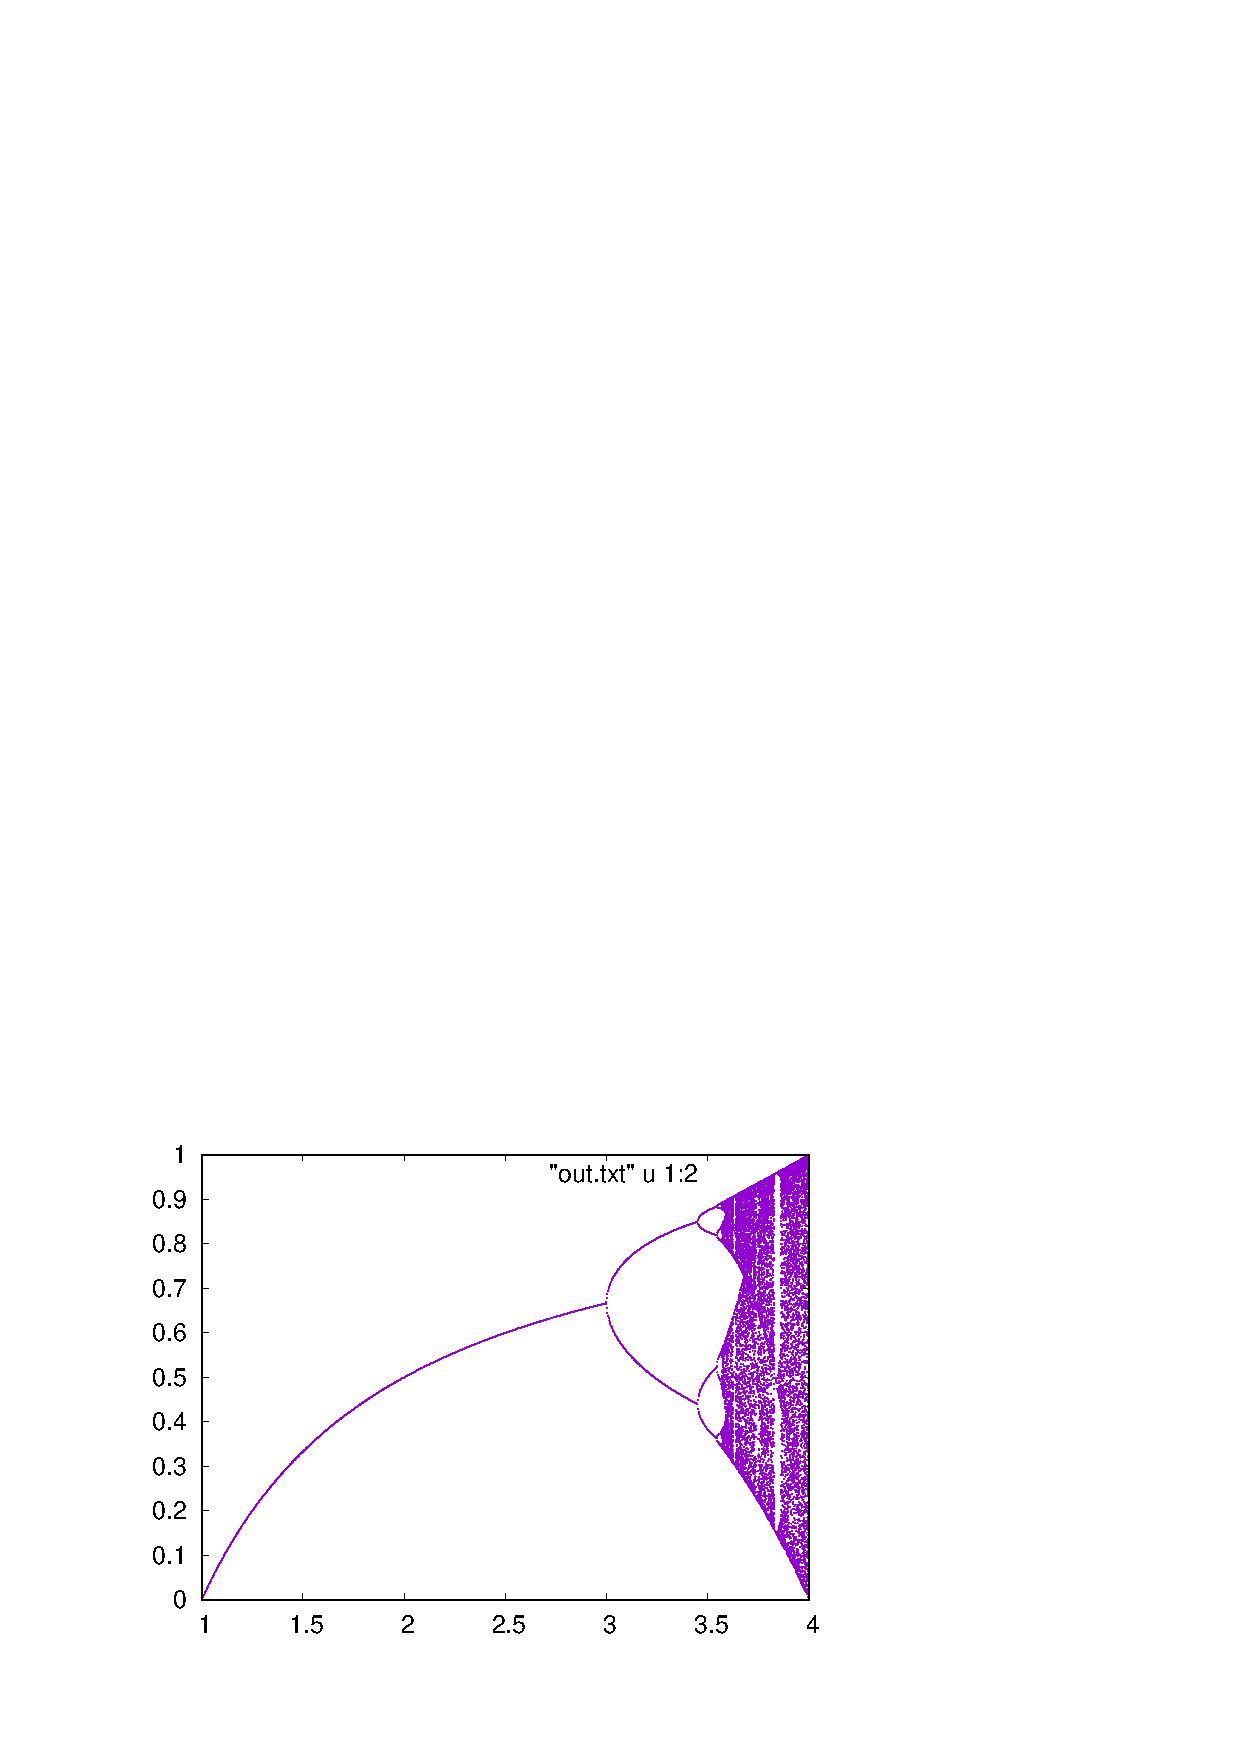
\includegraphics[clip, width=15cm]{6-2.jpg} 
  \label{fig:level}
 \end{center}
\end{figure}
\subsubsection{考察\\}
グラフを見るとわかるのですが,カオス的な振る舞いをしていることが確認できた。\\
実行結果からも一定の値に収束,周期的な振動を起こしていたことがわかる。\\



\end{document}
